\subsection{IMU Temperature Compensation}

There is a common saying that floats around the inertial sensor industry, "MEMS sensors are almost more useful thermometers than inertial sensing themselves!". This rings true in practice, and temperature compensation becomes a key part of making inertial sensors suitable for navigation applications. 

Unfortunately, the process for characterizing inertial sensor temperature sensitivity and follow-on compensation models are not standardized. Most processes are proprietary to the sensor manufacturers and most IEEE standards for specifying varying inertial sensor technologies \cite{IEEE_std_1293-2018,IEEE_std_1431-2004,IEEE_std_952-2020,IEEE_std_292-1969,IEEE_std_517-1974,IEEE_std_647-2006,IEEE_std_813-1988} seldom reference error in response to temperature. 

Without a standardized procedure, multiple academic papers such as \cite{9851744} will model all of the calibration parameters in \ref{eq: expanded IMU forward error model} as polynomial functions over temperature. A calibration procedure will be repeated many times at different temperatures to provide data for performing a polynomial fit. Many rate tables are equipped with ovens for this exact purpose and are considered necessary for high-grade sensors.

Figure \ref{fig: ideal and fictitious bias sensitivity to temperature} shows an example of how a temperature sensitivity affecting the bias of an accelerometer may appear after multiple rounds of testing.

\begin{figure}[h] 
	\centering
	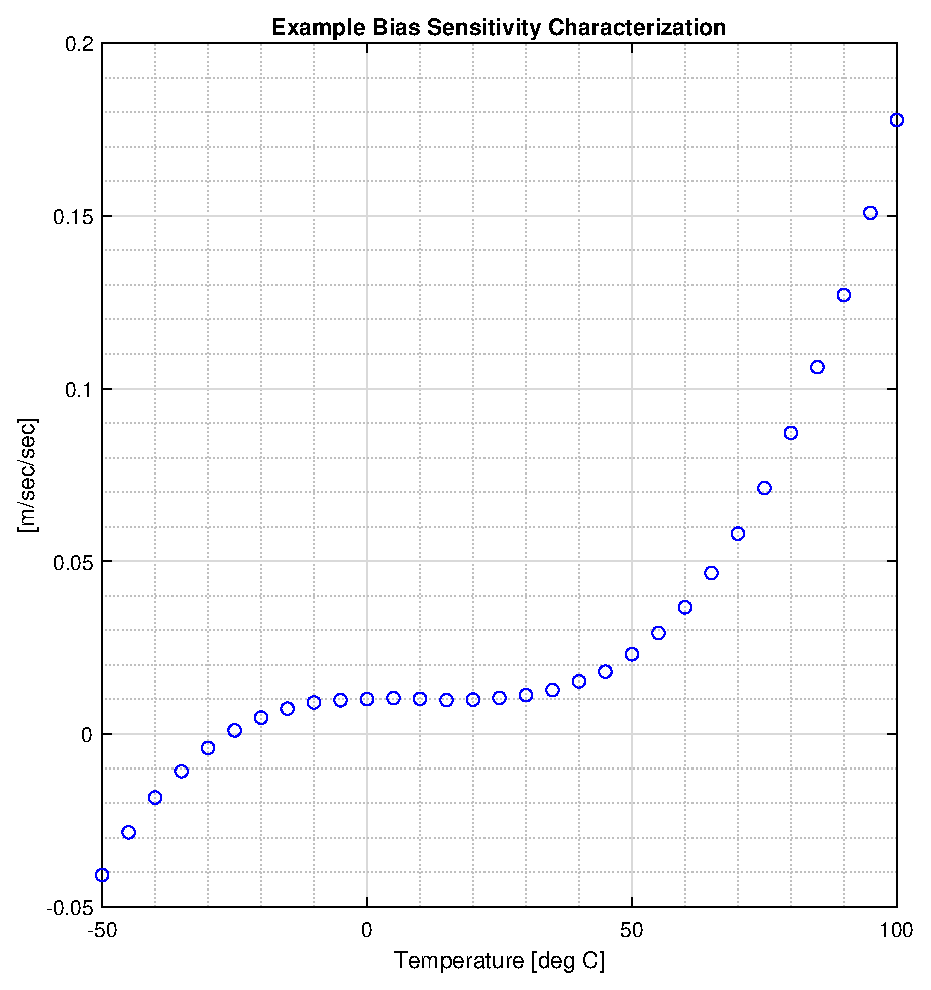
\includegraphics[width=0.65\textwidth]{./images/ideal_bias_response_to_temperature.eps}
	\caption{Ideal and Fictitious Bias Sensitivity to Temperature}
	\label{fig: ideal and fictitious bias sensitivity to temperature}
\end{figure}
\FloatBarrier

In practice however, it is rare to have the opportunity to collect so many data points over such a wide temperature range. It can take anywhere from thirty minutes to an hour per data point to heat or cool an IMU to a specific temperature before repeating a calibration cycle. In an inertial test laboratory (ITL) where both rate tables and technician time is limited, each collected data point becomes very costly. 

In light of these practical constraints, this paper aims to design experiments to characterize IMU temperature sensitivity through the lens of inverse problem techniques. This paper will consider a hypothetical scenario in which an ITL receives a new IMU to characterize. Experiment designs will consider how many data points must be collected, what degree of polynomials can be modeled, and how noise will impact the ability to estimate model parameters. 


methods

Consider a scenario in which an ITL receives a new IMU to characterize. Nothing is known about this IMU except for the information provided by its specification sheet. Performing a calibration procedure at an ambient temperature is trivial, however repeating the calibration procedure at other temperatures may take an entire day. Suppose that only one day is available for testing and in one day, the ITL is able to collect six data points. A data analyst needs to design an experiment to perform some form of polynomial regression with the available data, but there a few items for consideration.

\begin{itemize}
	\item From past experience, the data analyst knows that the degree for the polynomial of best fit could be anywhere from one to ten. 
	\item Each data point will be subject to an unknown amount of noise which will be modeled as zero-mean and Gaussian.
\end{itemize}